\documentclass[12pt]{beamer}
\usetheme{Darmstadt}
\usepackage{graphicx}
\usepackage[ngerman]{babel}
\usepackage[T1]{fontenc}
\usepackage[utf8]{inputenc}
\usepackage{tikz}
\usepackage[shadow,colorinlistoftodos]{todonotes}
\setbeamertemplate{footline}[frame number]

\newcommand{\cc}[1]{\includegraphics[height=4mm]{img/#1.png}}
\usepackage{ifthen}
\newcommand{\license}[2][]{\\#2\ifthenelse{\equal{#1}{}}{}{\\\scriptsize\url{#1}}}
\usepackage{textcomp}

%\setbeamercovered{transparent}

\pgfdeclareimage[height=.6cm]{c3d2logo}{./img/c3d2.pdf} 


\pgfdeclarelayer{foreground}
\pgfsetlayers{main,foreground}
\logo{\pgfputat{\pgfxy(-1,0)}{\pgfbox[center,base]{\pgfuseimage{c3d2logo}}}}


\title{Daten auf der Spur - Sicher im Netz}
\author{\small t3sserakt \& Thammi \\\large Chaos Computer Club Dresden}
\date{25.05.2018}

\begin{document}
\maketitle

\section*{Einleitung}
\subsection*{}

%%% -> thammi -> %%%

\begin{frame}
  \frametitle{Hacker}
  \begin{figure}
    \only<2>{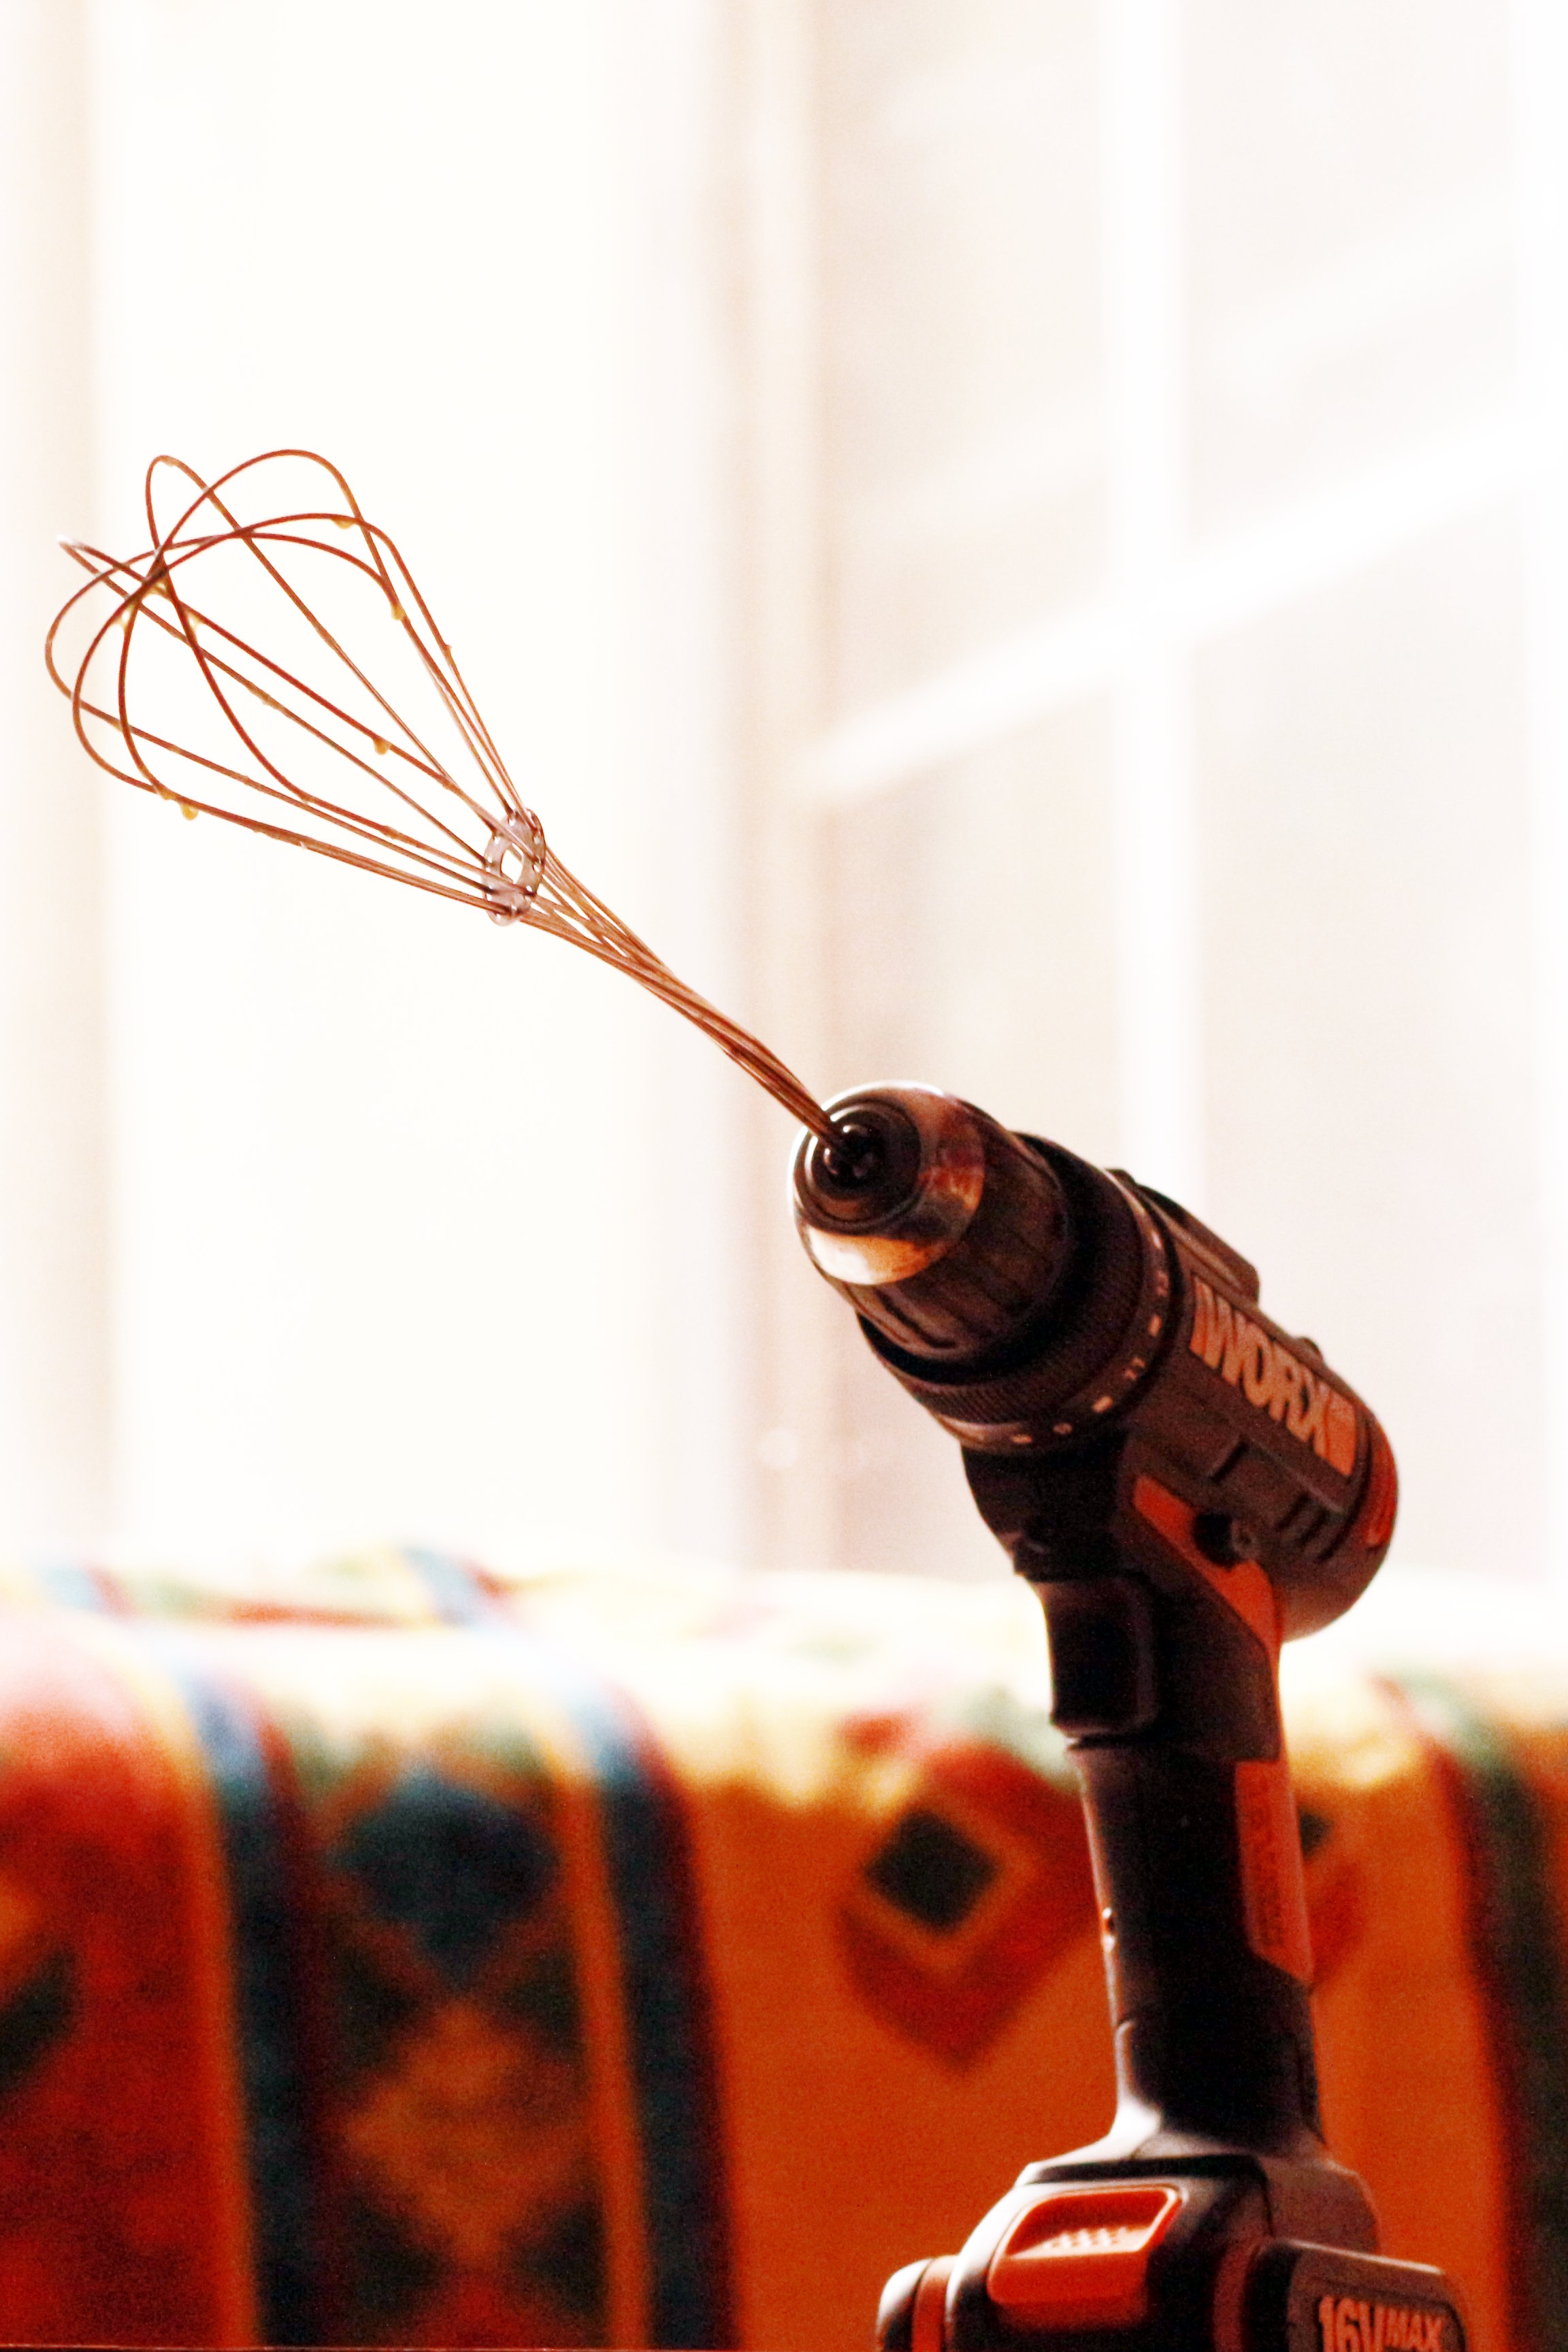
\includegraphics[height=0.7\textheight]{img/schneeschrauber.jpg}}
    \only<3>{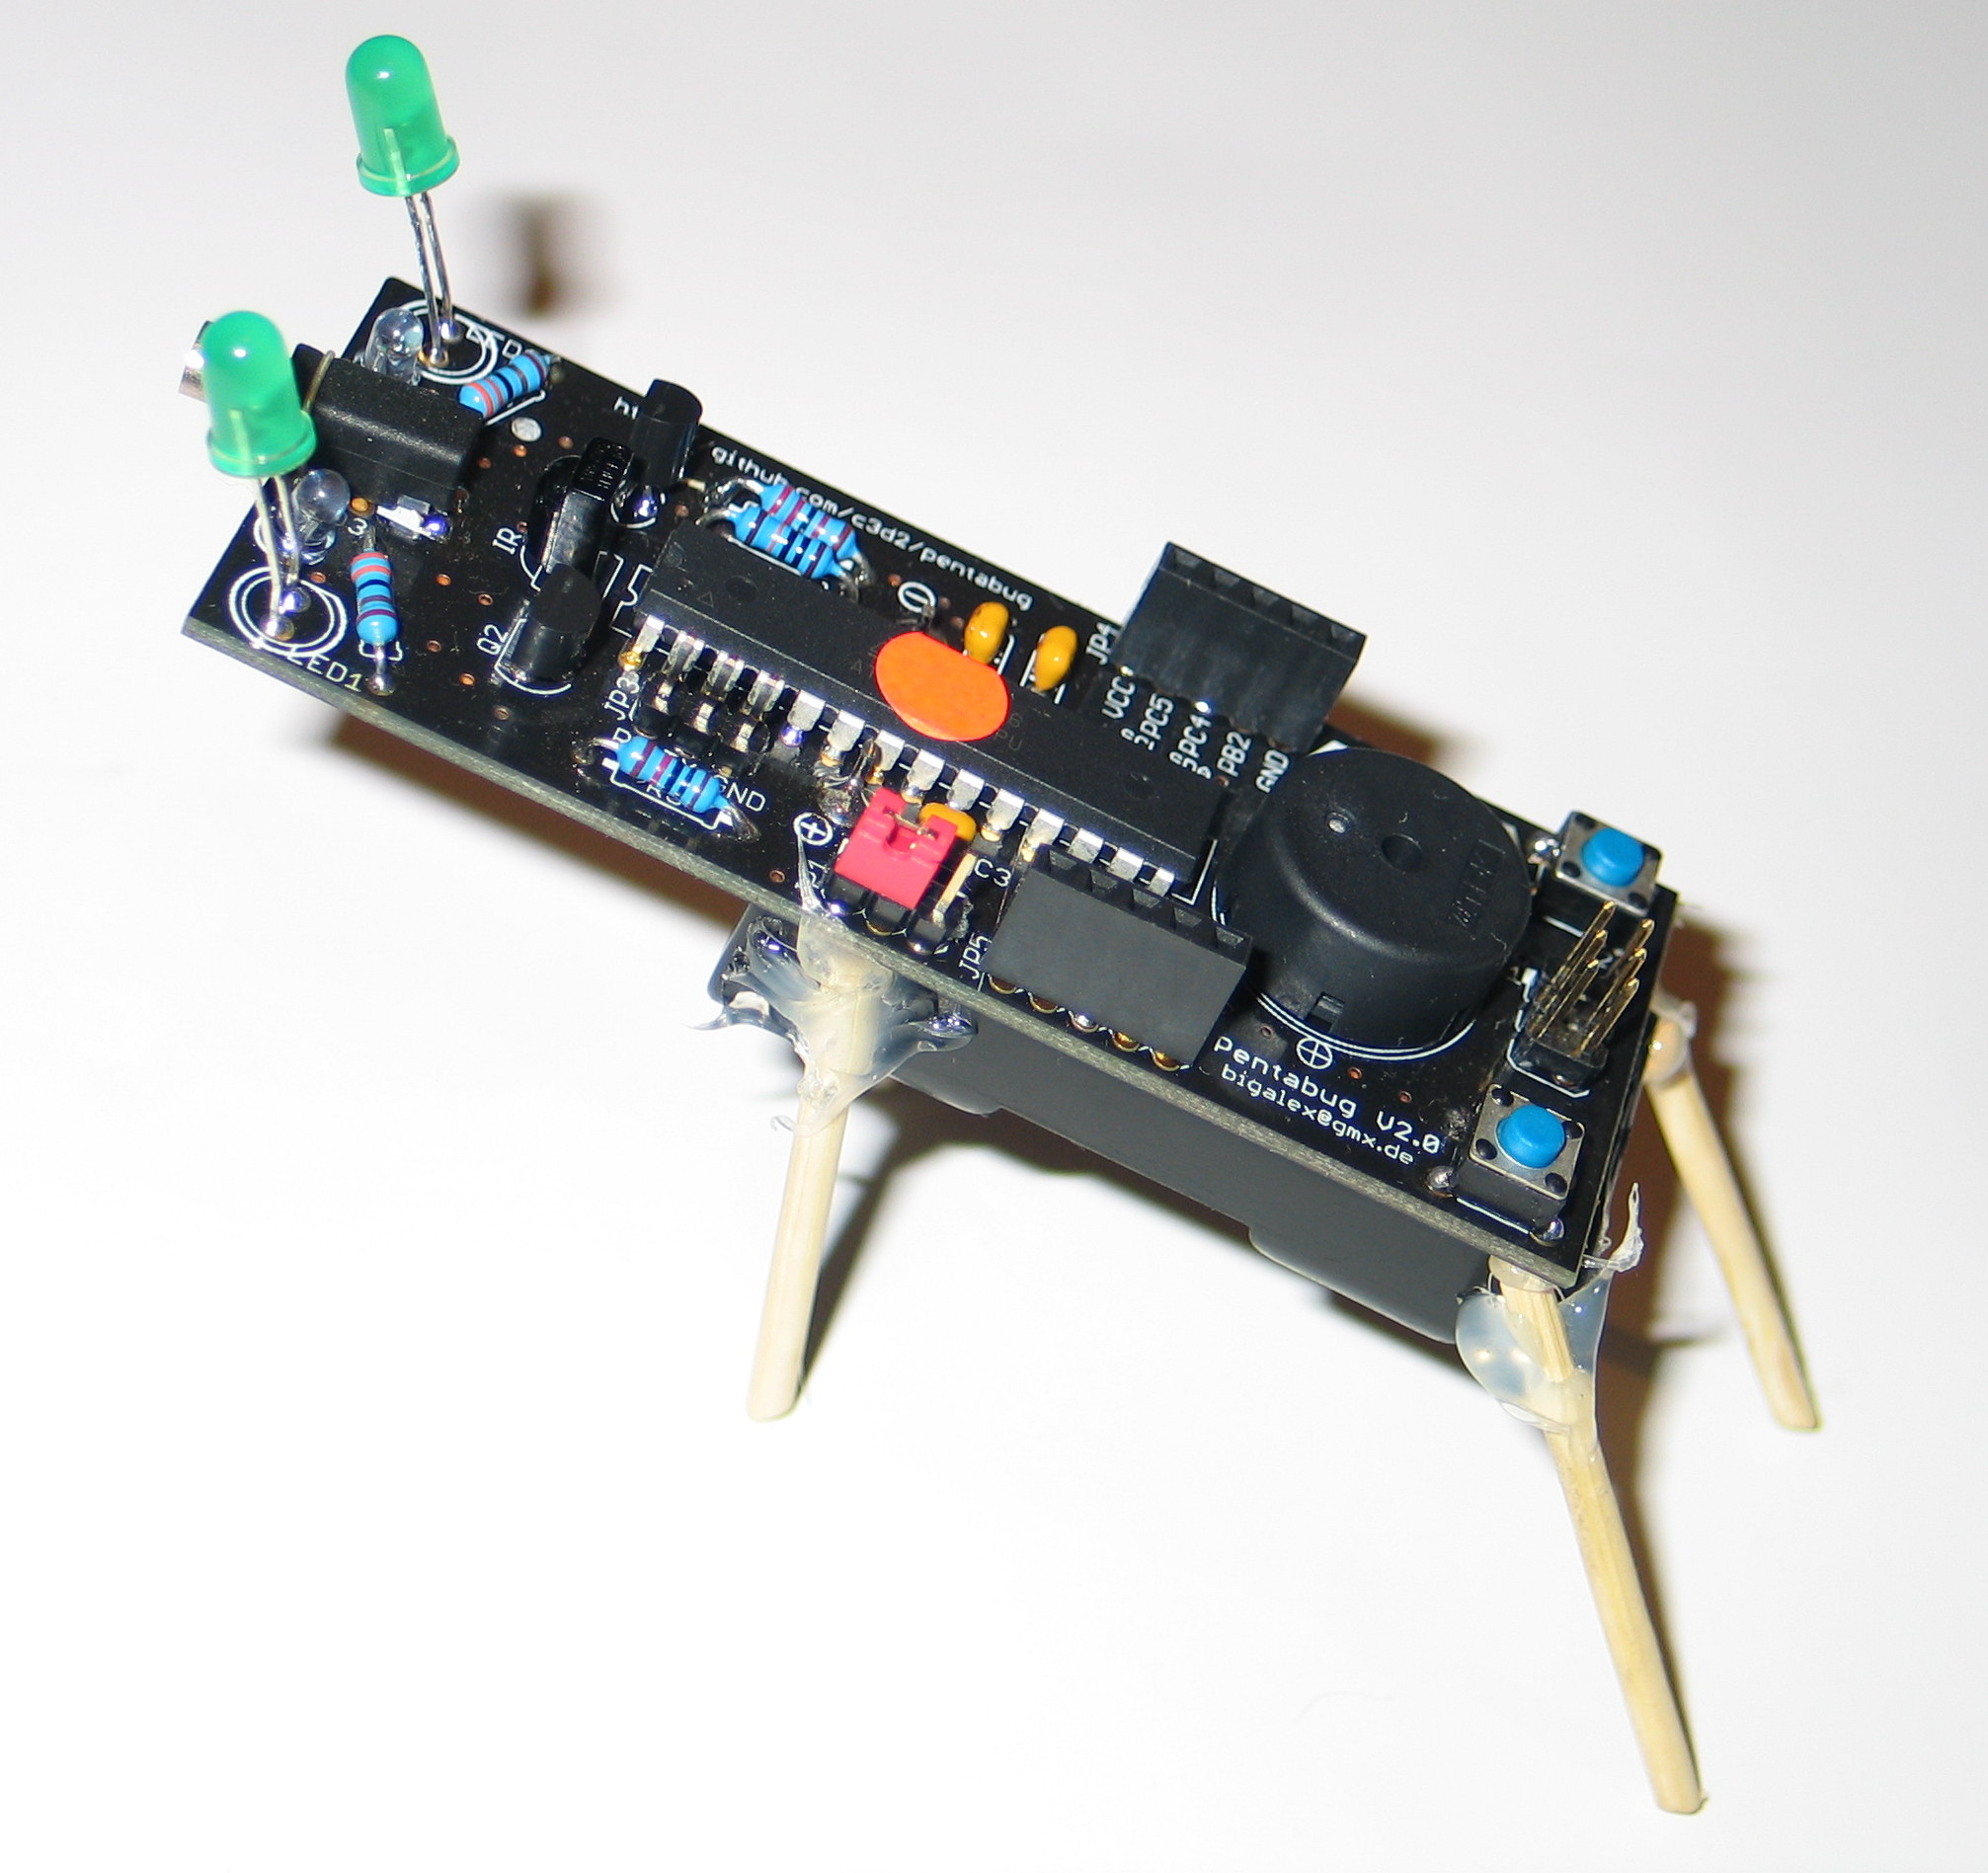
\includegraphics[height=0.7\textheight]{img/pentabug.jpg}}
  \end{figure}
\end{frame}

\begin{frame}
	\frametitle{Chaos Computer Club}
	\begin{center}
		
\includegraphics[height=0.2\textheight]{img/chaosknoten.png}
	\end{center}	
	\begin{itemize}
		\item Verein wurde 1981 gegründet
		\item Aktuell mehr als 6000 Mitglieder
		\item Datenspuren
		\item Radio und Podcasts
		\item Chaos macht Schule
	\end{itemize}
\end{frame}

\section{Forschertag}
\subsection{}

\begin{frame}
  \frametitle{Umfrage}
  \begin{center}
    \huge Wie oft seid ihr im Internet?
  \end{center}
\end{frame}

\begin{frame}
  \frametitle{Internet}
  \begin{center}
    \only<2>{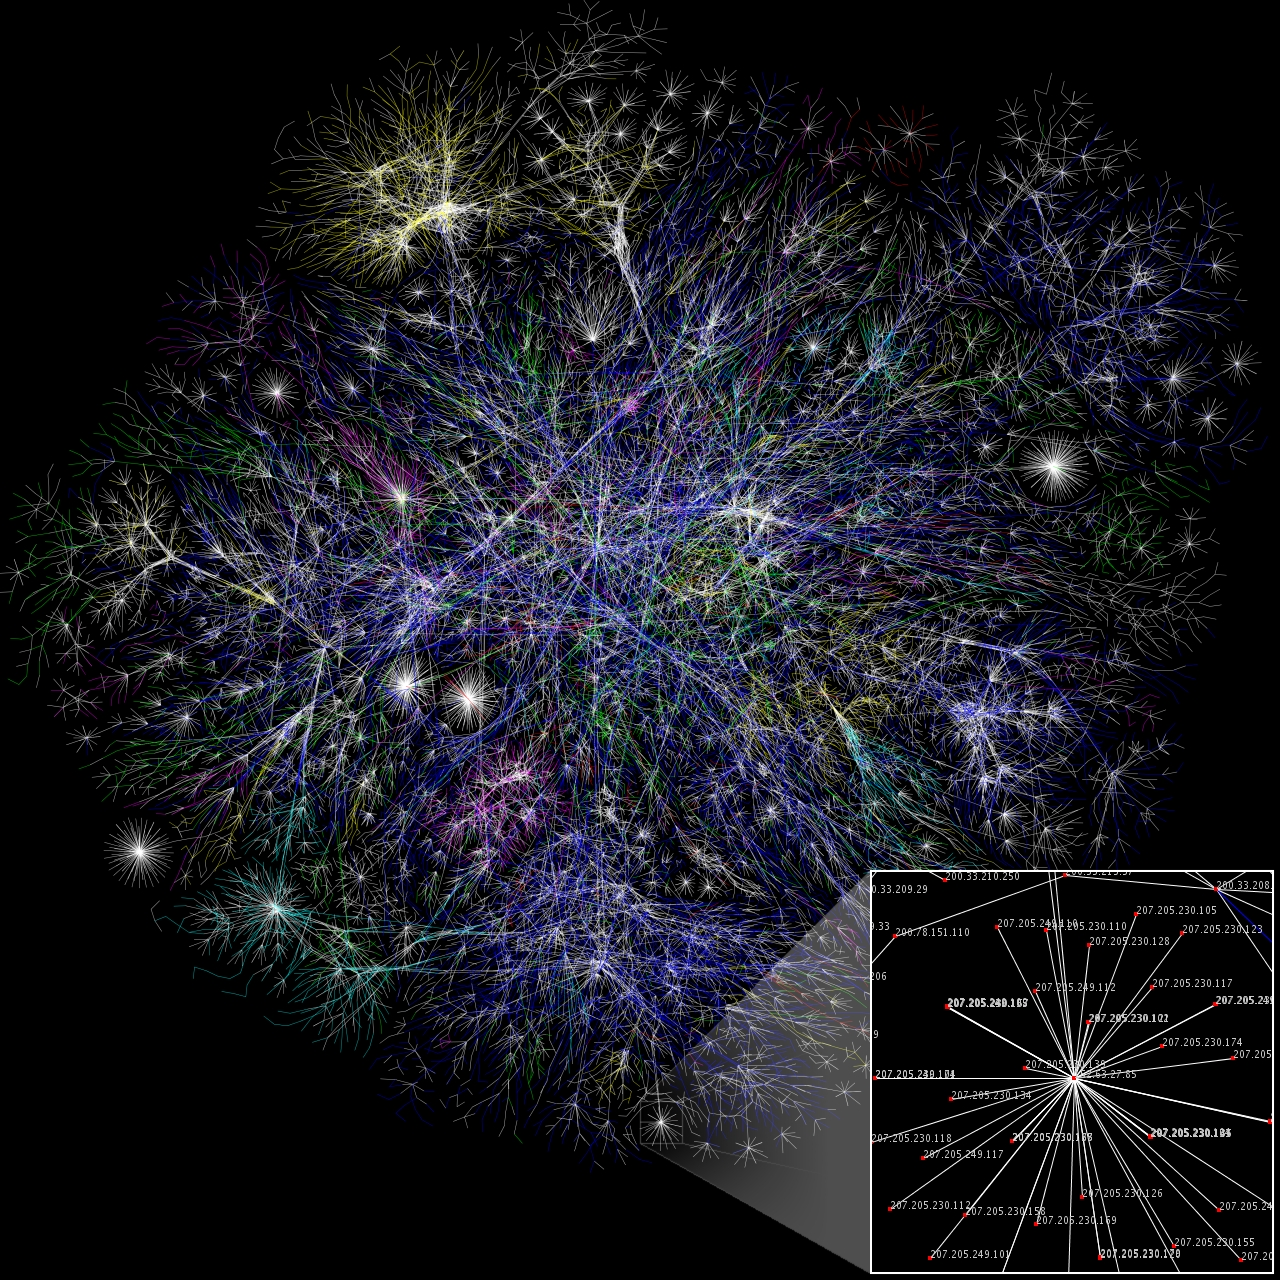
\includegraphics[height=0.7\textheight]{img/internet_0.jpg}}
    \only<3>{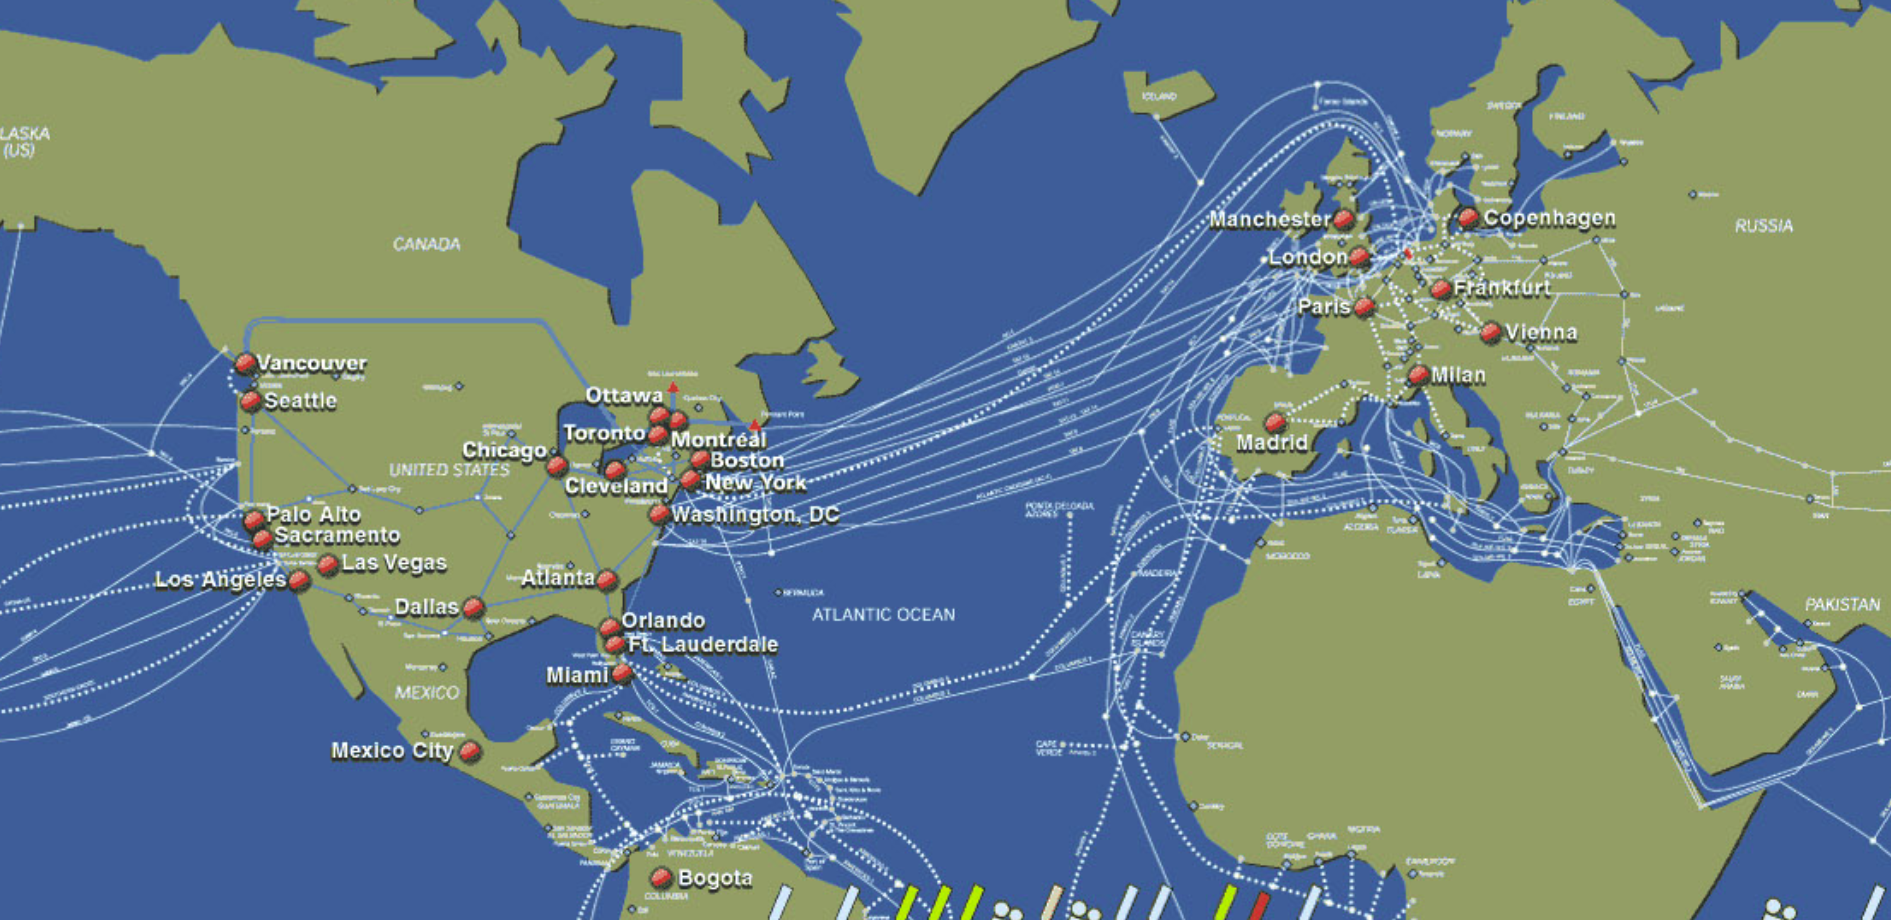
\includegraphics[height=0.7\textheight]{img/internet_1.png}}
    \only<4>{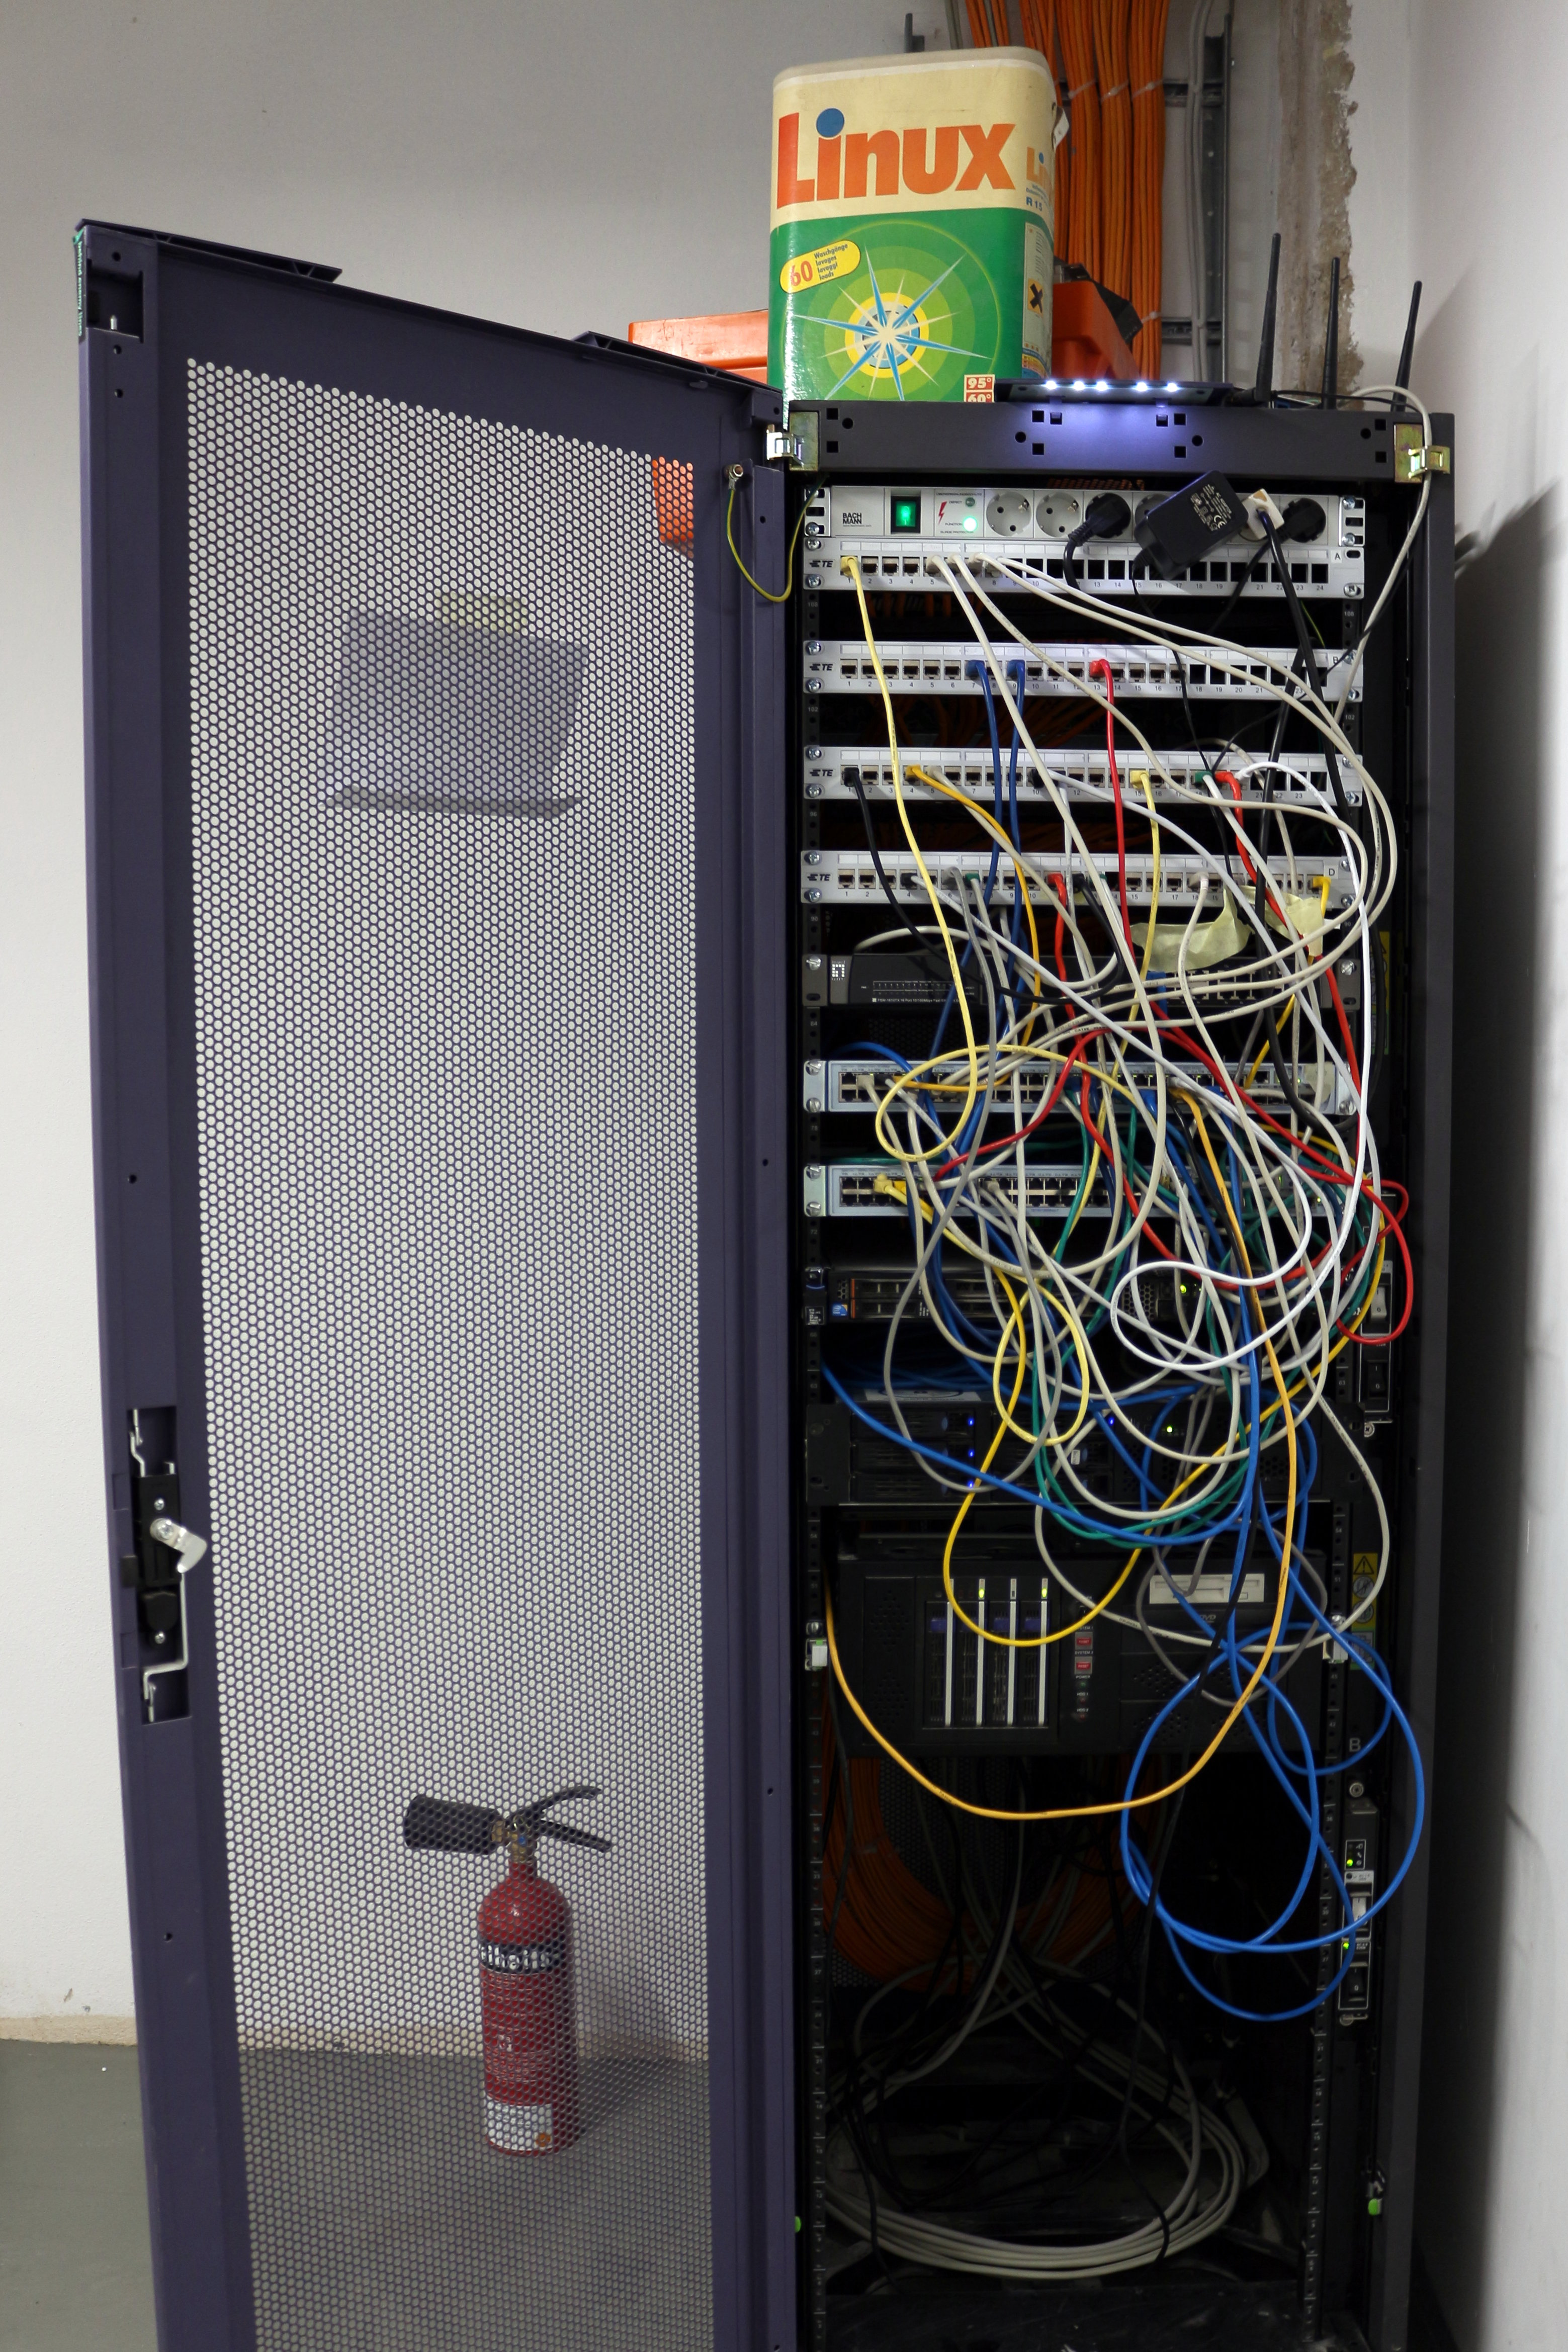
\includegraphics[height=0.7\textheight]{img/rack.jpg}}
  \end{center}
\end{frame}

\begin{frame}
    \frametitle{Kindernet}
    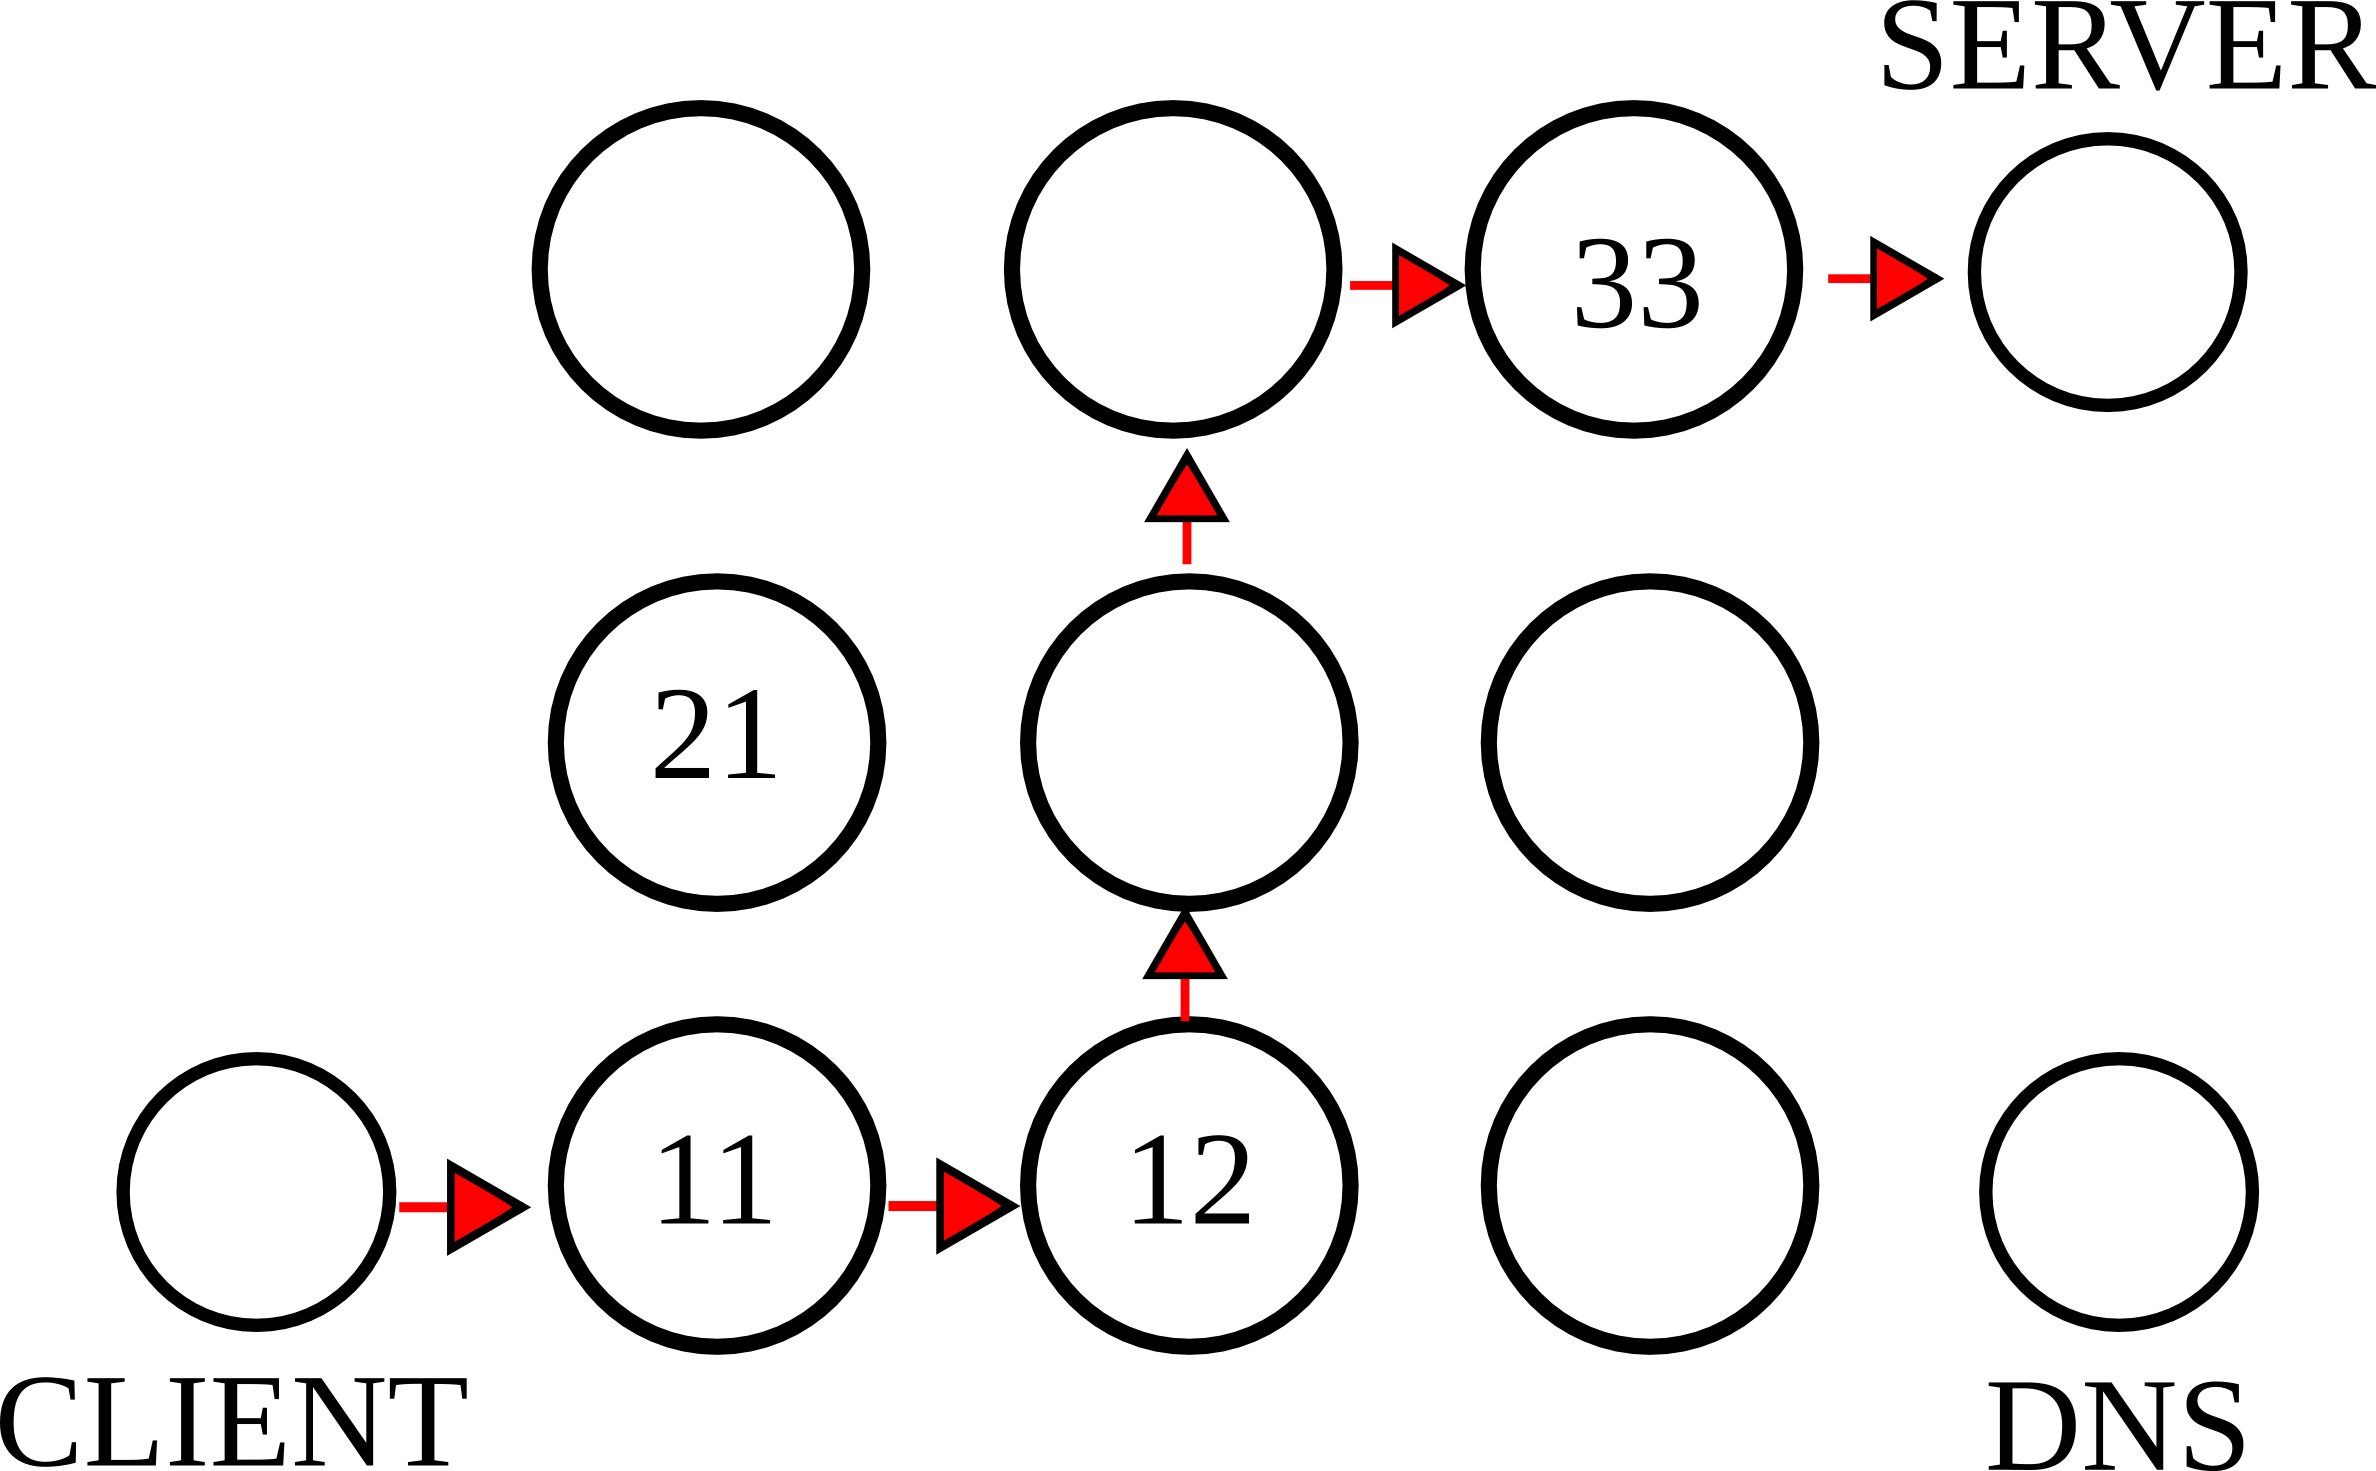
\includegraphics[height=0.6\textheight]{img/kindernet.png}
\end{frame}

\begin{frame}
  \frametitle{Traceroute}
  \begin{figure}
    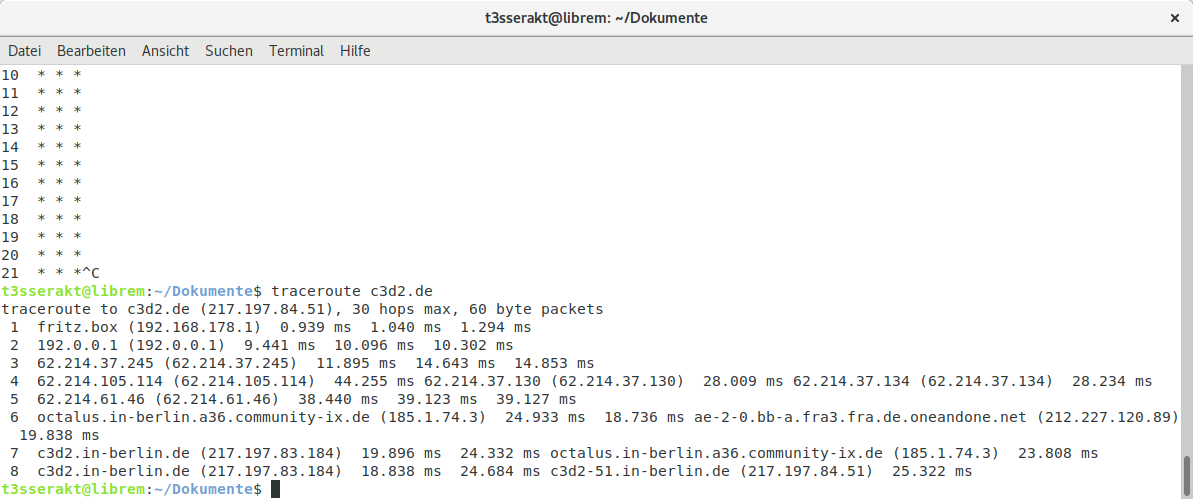
\includegraphics[height=0.5\textheight]{img/trace.png}
  \end{figure}
\end{frame}

\begin{frame}
  \frametitle{Verschlüsselung}
  \begin{center}
    \only<1>{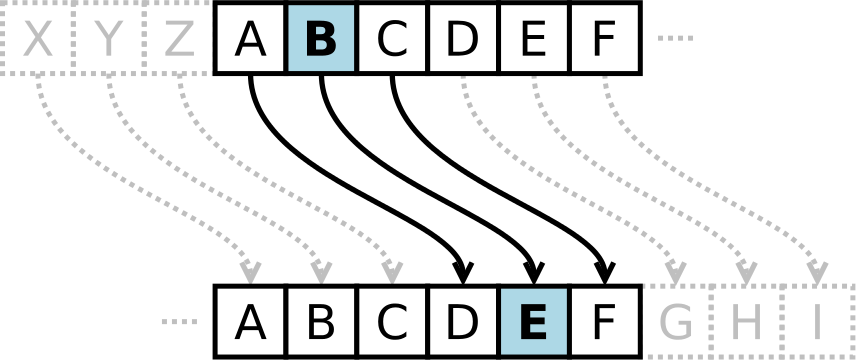
\includegraphics[height=0.5\textheight]{img/caesar.png}}
    \only<2>{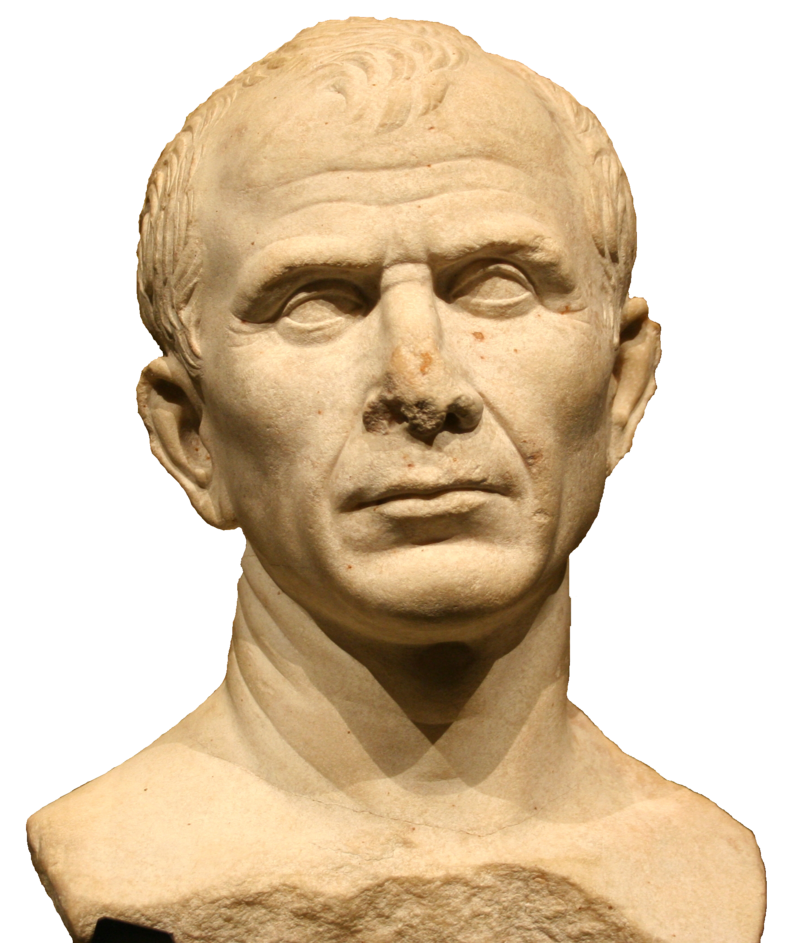
\includegraphics[height=0.7\textheight]{img/caesar_bueste.png}}
  \end{center}
\end{frame}

\begin{frame}
  \frametitle{HTTPS}
  \begin{center}
    \only<1>{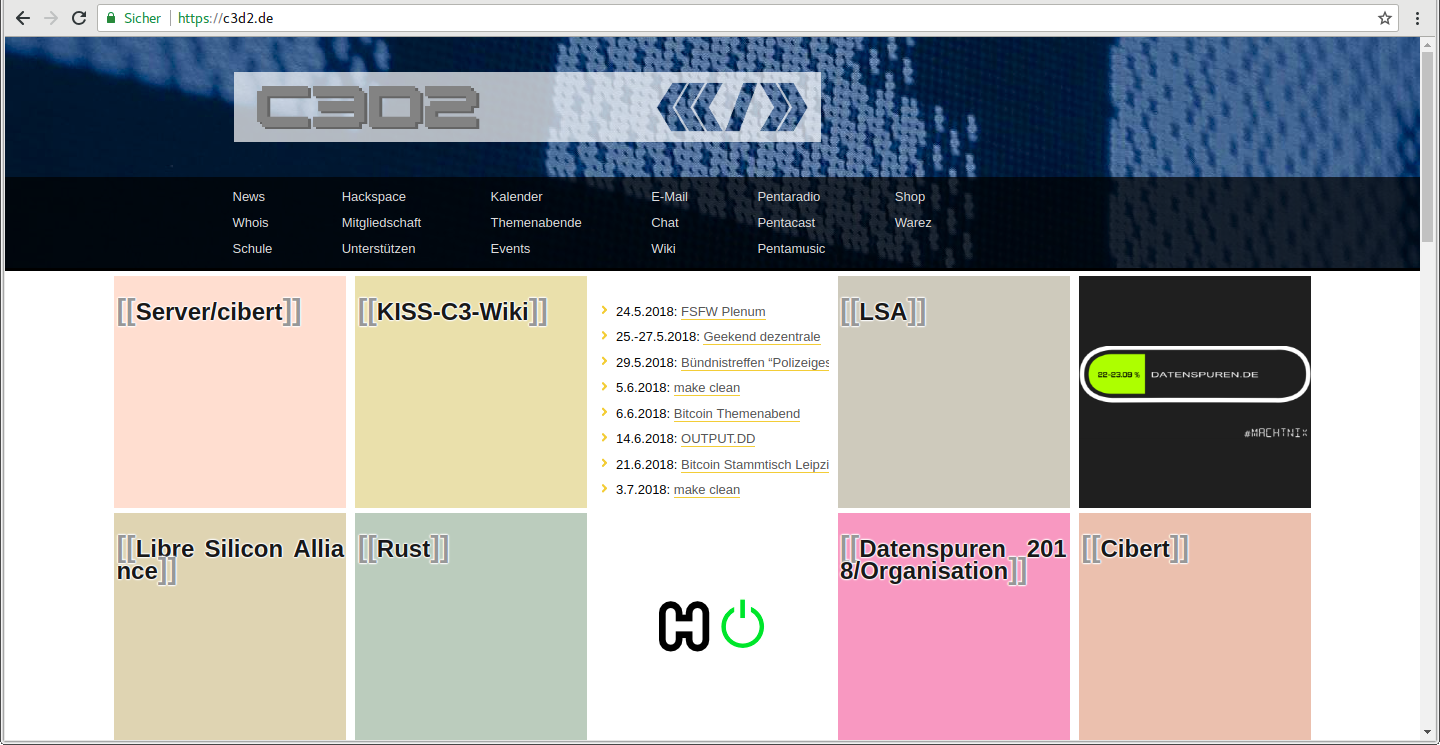
\includegraphics[height=0.6\textheight]{img/website_a.png}}
    \only<2>{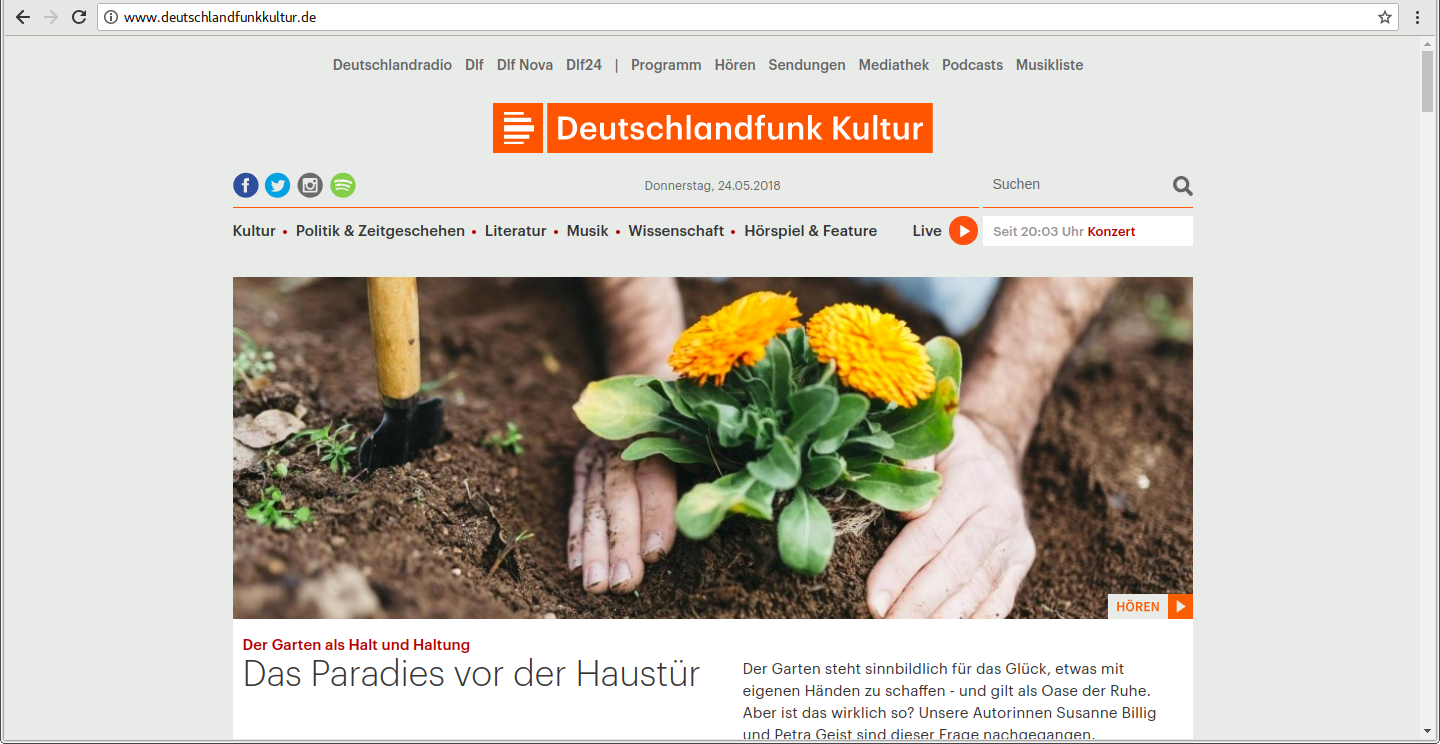
\includegraphics[height=0.6\textheight]{img/website_b.png}}
    \only<3>{
\includegraphics[height=0.3\textheight]{img/website_a_zoom.png}}
    \only<4>{
\includegraphics[height=0.3\textheight]{img/website_b_zoom.png}}
  \end{center}
\end{frame}

\end{document}
